\documentclass{beamer}
 
\usepackage[utf8]{inputenc}

\usetheme{Madrid}
\usecolortheme{default}

\usepackage[qm]{qcircuit}
\usepackage{bibentry}
\usepackage{tikz,tikz-cd}












\usepackage{physics}
\usepackage{amsmath}
\usepackage{amsfonts}
\usepackage{esint}
\usepackage{bbold}
\usepackage{mathtools}
\usepackage{dsfont}
\usepackage{amsthm}
\usepackage{bbm}
\usepackage{amssymb}
\theoremstyle{definition}
\newtheorem{defn}{Definition}[section]
\newtheorem{prop}{Properties}[section]
\newtheorem{rmk}{Remark}[section]
\newtheorem{exmp}{Example}[section]
\newtheorem{prob}{Problem}[section]
\newtheorem{sln}{Solution}[section]
\newtheorem{thm}{Theorem}[section]
\newtheorem*{prob*}{Problem}
\newtheorem*{sln*}{Solution}
\usepackage{empheq}
\usepackage{tensor}
\usepackage{hyperref}
\usepackage{xcolor}

\newcommand{\R}{\mathbb{R}}
\newcommand{\F}{\mathcal{F}}
\newcommand{\p}{\partial}

\newcommand{\V}{\mathbf{V}}
\newcommand{\W}{\mathbf{W}}
\newcommand{\Z}{\mathbf{Z}}
\newcommand{\Y}{\mathbf{Y}}
\newcommand{\U}{\mathbf{U}}
\newcommand{\X}{\mathbf{X}}

\newcommand{\A}{\mathcal{A}}
\newcommand{\B}{\mathcal{B}}

\newcommand{\xpan}{\text{span}}

\newcommand{\lag}{\mathcal{L}}

\newcommand{\J}{\mathbf{J}}

\newcommand{\M}{\mathcal{M}}

\newcommand{\lp}{\left(}
\newcommand{\rp}{\right)}

\newcommand{\lb}{\left[}
\newcommand{\rb}{\right]}

\newcommand{\lc}{\left\{}
\newcommand{\rc}{\right\}}

\newcommand{\K}{\mathcal{K}}

\newcommand{\N}{\mathcal{N}}

\newcommand{\E}{\mathcal{E}}

\newcommand{\ima}{\text{Im}}
\newcommand{\lin}{\overset{\text{linear}}{\longrightarrow}}
\newcommand{\T}{\mathcal{T}}
\newcommand{\poly}{\mathbb{P}}
\newcommand{\s}{\mathcal{S}}

\newcommand{\gives}{\rotatebox[origin=c]{180}{$\Rsh$}	}


\newcommand{\bigzero}{\mbox{\normalfont\Large\bfseries 0}}
\newcommand{\rvline}{\hspace*{-\arraycolsep}\vline\hspace*{-\arraycolsep}}




 
 
%Information to be included in the title page:
\title{Matrices in Quantum Computing}
\author[Huan Q. Bui] % (optional)
{Huan Q. Bui}

\institute[Colby College] % (optional)
{
	
	Matrix Analysis
	\and
	Professor Leo Livshits
}
\date{CLAS, May 2, 2019}
 
%\logo{
\includegraphics[height=0.3cm]{colby.png}}
 
\begin{document}
 
\frame{\titlepage}

%%%%%%%%%%%%%%%%%%%%%%%%%%%%%%%%%%%%%%%%%%%%%%%%%%%%%%%%%%%%%%%%%%%%%%%%%



\begin{frame}[fragile]
\begin{center}
	$\,$\Qcircuit @C=.7em @R=.4em  {
		\lstick{a: \ket{0}} & \qw & \qw & \targ & \meter & \qw \\
		\lstick{b: \ket{0}} & \qw & \gate{H} & \ctrl{-1}& \meter & \qw 
	}
\end{center}
\end{frame}


%%%%%%%%%%%%%%%%%%%%%%%%%%%%%%%%%%%%%%%%%%%%%%%%%%%%%%%%%%%%%%%%%%%%%%%%%

 
\begin{frame}
\frametitle{Presentation layout}
\tableofcontents
\end{frame}

%%%%%%%%%%%%%%%%%%%%%%%%%%%%%%%%%%%%%%%%%%%%%%%%%%%%%%%%%%%%%%%%%%%%%%%%%

\section{Background}

\begin{frame}
\frametitle{Background}
%\pause
\begin{center}
	$\,$\Qcircuit @C=.7em @R=.4em  {
		\lstick{a: \ket{0}} & \qw & \qw & \targ & \meter & \qw \\
		\lstick{b: \ket{0}} & \qw & \gate{H} & \ctrl{-1}& \meter & \qw 
	}
\end{center}
\pause
Components:
\begin{enumerate}
	\pause
	\item Quantum bits - Qubits
	\pause
	\item Quantum gates: single and multiple-qubit gates
	\pause
	\item Measurement
\end{enumerate}
\end{frame}


\begin{frame}
\frametitle{Quantum Bits - Qubits}
\begin{figure}[h!]
	\centering
	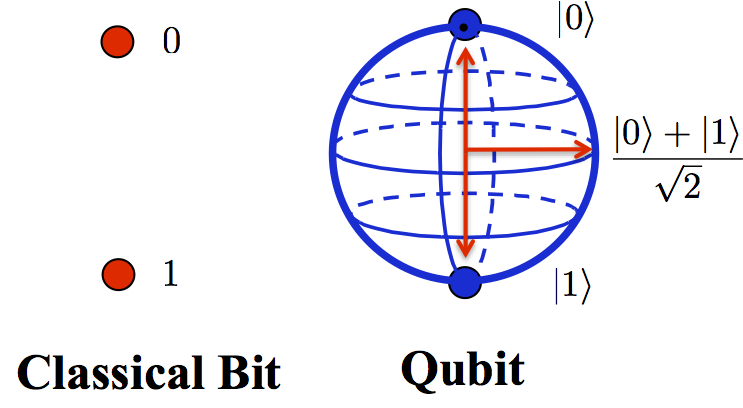
\includegraphics[scale=0.45]{atom1.png}
\end{figure}
\pause
$$
a\begin{bmatrix}
1\\0
\end{bmatrix}
+
b\begin{bmatrix}
0\\1
\end{bmatrix}
\hspace{0.5cm}
\pause
\vert a \vert^2 + \vert b\vert^2 = 1 $$ 
\pause
$$ \boxed{a\ket{0} + b\ket{1}} $$
\end{frame}

%%%%%%%%%%%%%%%%%%%%%%%%%%%%%%%%%%%%%%%%%%%%%%%%%%%%%%%%%%%%%%%%%%%%%%%%%

\begin{frame}
\frametitle{Quantum Gates}
\pause
$\rightarrow$ linear transformations on one or many qubits.\\
\pause 
$\,$\\
Example: Hadamard gate.
\begin{align*}
 H \equiv \frac{1}{\sqrt{2}}\begin{bmatrix}
1&1\\1&-1
\end{bmatrix}
\end{align*}
\pause
\begin{center}
	$\,$\Qcircuit @C=.7em @R=.4em  {
		\lstick{a: \ket{0}} & \qw & \qw & \targ & \meter & \qw \\
		\lstick{b: \ket{0}} & \qw & \gate{H} & \ctrl{-1}& \meter & \qw 
	}
\end{center}
\pause
What does $H$ do to, say  $\ket{0}$?
\pause
\begin{align*}
H\ket{0} \onslide<7->{= H\begin{bmatrix}
1\\0
\end{bmatrix} \onslide<8->{= \frac{1}{\sqrt{2}}\begin{bmatrix}
1\\1
\end{bmatrix} \onslide<9->{ = \frac{1}{\sqrt{2}}\ket{0} + \frac{1}{\sqrt{2}}\ket{1}}}}
\end{align*}


\end{frame}

%%%%%%%%%%%%%%%%%%%%%%%%%%%%%%%%%%%%%%%%%%%%%%%%%%%%%%%%%%%%%%%%%%%%%%%%%

\begin{frame}
\frametitle{Multiple Qubits}
\pause
$\hspace{1cm}$Qubit 1: $a\ket{0} + b\ket{1} = \begin{bmatrix} a\\b \end{bmatrix} \hspace{0.5cm}$ Qubit 2: $c\ket{0} + d\ket{1} = \begin{bmatrix}
c\\d
\end{bmatrix}$




\pause
\begin{align*}
\begin{bmatrix}
a\\b
\end{bmatrix}
\boxtimes
\begin{bmatrix}
c\\d
\end{bmatrix} = \begin{bmatrix}
a\begin{bmatrix}
c\\d
\end{bmatrix}\\
b\begin{bmatrix}
c\\d
\end{bmatrix}
\end{bmatrix}
=
\begin{bmatrix}
ac\\ad\\bc\\bd
\end{bmatrix}.
\end{align*}
\end{frame}

\begin{frame}
\frametitle{Multiple Qubits}
Do this for the basis states 
\begin{align*}
\ket{0}\boxtimes \ket{0}
=
\begin{bmatrix}
1\\0\\0\\0
\end{bmatrix}\,\,\ket{0}\boxtimes \ket{1}
=
\begin{bmatrix}
0\\1\\0\\0
\end{bmatrix}\,\,\ket{1}\boxtimes \ket{0}
=
\begin{bmatrix}
0\\0\\1\\0
\end{bmatrix}\,\, \ket{1}\boxtimes \ket{1}
=
\begin{bmatrix}
0\\0\\0\\1
\end{bmatrix}
\end{align*}
\pause
Notation:
\begin{align*}
\ket{00} = \ket{0} \boxtimes \ket{0}\hspace{1cm}&
\ket{01} = \ket{0} \boxtimes \ket{1}\\
\ket{10} = \ket{1} \boxtimes \ket{0}\hspace{1cm}&
\ket{11} = \ket{1} \boxtimes \ket{1}
\end{align*}
\pause
Can see that we have a basis for describing the combined state.
\begin{align*}
\begin{bmatrix}
a\\b
\end{bmatrix}
\boxtimes
\begin{bmatrix}
c\\d
\end{bmatrix} = ac\ket{00} + ad\ket{01} + bc\ket{10} + bd\ket{11}. 
\end{align*}

\end{frame}



%%%%%%%%%%%%%%%%%%%%%%%%%%%%%%%%%%%%%%%%%%%%%%%%%%%%%%%%%%%%%%%%%%%%%%%%%



\section{Matrices in an entanglement circuit}

\begin{frame}
\frametitle{Elementariness \& Entanglement}
\pause
Not all combined states can be written as $ \ket{a}\boxtimes \ket{b} \leftarrow \textbf{Elementary}$.\\
$\,$\\
\pause
Ex: $p(x)\cdot q(y)$ is a ``combined state.'' But there are NO $p(x), q(y)$ s.t. $$p(x)\cdot q(y) = xy + 1,$$ even though $xy + 1$ is a legitimate ``combined state.''\\
\pause
$\,$\\
Back to qubits. Consider this combined state:\pause
\begin{align*}
\frac{1}{\sqrt{2}}\begin{bmatrix}
1\\0\\0\\1
\end{bmatrix} \onslide<6->{= \frac{1}{\sqrt{2}}\ket{00} + \frac{1}{\sqrt{2}}\ket{11} \onslide<7->{ \longrightarrow \textbf{Entangled}}}
\end{align*}

\end{frame}

%%%%%%%%%%%%%%%%%%%%%%%%%%%%%%%%%%%%%%%%%%%%%%%%%%%%%%%%%%%%%%%%%%%%%%%%%

\begin{frame}
\frametitle{Kronecker Product}
\pause
$\A$ is a matrix acting on $\ket{a}$, $\B$ on $\ket{b}$ 
\pause
\begin{align*}
\A\ket{a} \boxtimes \mathcal{B}\ket{b} = (\A \otimes \mathcal{B})(\ket{a} \boxtimes \ket{b})
\end{align*}
\pause
$\otimes:$ Kronecker product, of two matrices. \\
\pause
$\,$\\
If
\begin{align*}
\A = \begin{bmatrix}
m & n \\ o & p
\end{bmatrix}
\hspace{0.5cm}\text{ and }
\mathcal{B} = \begin{bmatrix}
q & r & s \\ t & u & v \\ w & x & y
\end{bmatrix}
\end{align*} 

\end{frame}


\begin{frame}
\frametitle{Kronecker Product}
then
\begin{align*}
\A \otimes \mathcal{B} 
\onslide<2->{
&= \begin{bmatrix}
m
\onslide<3->{\begin{bmatrix}
q & r & s \\ t & u & v \\ w&x&y
\end{bmatrix}} & n\onslide<4->{\begin{bmatrix}
q & r & s \\ t & u & v \\ w&x&y
\end{bmatrix}}\\
o\onslide<5->{\begin{bmatrix}
q & r & s \\ t & u & v \\ w&x&y
\end{bmatrix}} & p\onslide<6->{\begin{bmatrix}
q & r & s \\ t & u & v \\ w&x&y
\end{bmatrix}}
\end{bmatrix}\\
\onslide<7->{
&=
\begin{bmatrix}
mq & mr & ms & nq & nr & ns\\
mt & mu & mv & nt & nu & nv\\
mw & mx & ms & nw & nx & ny\\
oq & or & os & pq & pr & ps\\
ot & ou & ov & pt & pu & pv\\
ow & ox & oy & pw & px & py\\
\end{bmatrix}}}
\end{align*}
\end{frame}

\begin{frame}
\frametitle{Kronecker Product}
Check that $I\ket{0}\boxtimes H\ket{0} = (I\otimes H)\ket{00}$:
\begin{center}
	$\,$\Qcircuit @C=.7em @R=.4em  {
		\lstick{a: \ket{0}} & \qw & \qw & \targ & \meter & \qw \\
		\lstick{b: \ket{0}} & \qw & \gate{H} & \ctrl{-1}& \meter & \qw 
	}
\end{center}
\pause
LHS: 
\begin{align*}
I\ket{0} \boxtimes H\ket{0} \onslide<3->{&= \onslide<3->{\begin{bmatrix}
1 & 0 \\  0 & 1
\end{bmatrix}\begin{bmatrix}
1 \\ 0
\end{bmatrix} \boxtimes \frac{1}{\sqrt{2}}\begin{bmatrix}
1 & 1\\ 1 & -1
\end{bmatrix}\begin{bmatrix}
0 \\ 1
\end{bmatrix}\\
\onslide<4->{&= \begin{bmatrix}
1 \\ 0
\end{bmatrix} \boxtimes \frac{1}{\sqrt{2}}\begin{bmatrix}
1 \\ 1
\end{bmatrix} \\
\onslide<5->{&= \frac{1}{\sqrt{2}}\begin{bmatrix}
1\\1\\0\\0
\end{bmatrix}}}}}
\end{align*}
\end{frame}


\begin{frame}
\frametitle{Kronecker Product}
Check that $I\ket{0}\boxtimes H\ket{0} = (I\otimes H)\ket{00}$:\pause\\
$\,$\\
RHS:
\pause
\begin{align*}
(I \otimes H)\ket{00} \onslide<3->{= \begin{bmatrix}
\frac{1}{\sqrt{2}}\begin{bmatrix}
1&1\\1&-1
\end{bmatrix} & \mathcal{O}\\
\mathcal{O} & \frac{1}{\sqrt{2}}\begin{bmatrix}
1&1\\1&-1
\end{bmatrix} 
\end{bmatrix}\begin{bmatrix}
1\\0\\0\\0
\end{bmatrix} \onslide<4->{= \frac{1}{\sqrt{2}}\begin{bmatrix}
1\\1\\0\\0
\end{bmatrix}}}
\end{align*}
\end{frame}



%%%%%%%%%%%%%%%%%%%%%%%%%%%%%%%%%%%%%%%%%%%%%%%%%%%%%%%%%%%%%%%%%%%%%%%%%

\begin{frame}
\frametitle{Some properties \& Elementariness revisited}
\pause
$\otimes $ and $\boxtimes $ are very much alike. 
\pause
\begin{enumerate}
	\item Bilinear
	\pause
	\item Distributive. 
	\pause
	\begin{align*}
	\begin{bmatrix}
	a\\b
	\end{bmatrix}
	\boxtimes
	\begin{bmatrix}
	c\\d
	\end{bmatrix} \onslide<6->{&= (a\ket{0} + b\ket{1})\boxtimes (c\ket{0} + d\ket{1})\\
	\onslide<7->{
	&= ac\ket{00} + ad\ket{01} + bc\ket{10} + bd\ket{11}. }}
	\end{align*}
	\onslide<8->{
	\item Associative
	\onslide<9->{
	\item NOT commutative. \onslide<10->{ Ex: $\ket{01} \neq \ket{10}$.
	\onslide<11->{
	\item Elementariness.}}}}
	
\end{enumerate}
\end{frame}



\begin{frame}
\frametitle{Some properties and Elementariness revisited}
\pause
Ex: 
\begin{center}
	$\,$\Qcircuit @C=.7em @R=.4em  {
		\lstick{a: \ket{0}} & \qw & \qw & \targ & \meter & \qw \\
		\lstick{b: \ket{0}} & \qw & \gate{H} & \ctrl{-1}& \meter & \qw 
	}
\end{center}
\pause
The Control-NOT gate:
\pause
	\begin{align*}
CNOT_b = \begin{bmatrix}
1 & 0 & 0 & 0\\
0 & 0 & 0 & 1\\
0 & 0 & 1 & 0\\
0 & 1 & 0 & 0
\end{bmatrix} \hspace{0.5cm} \onslide<5-> {\longrightarrow \begin{cases}
\ket{00} \to \ket{00}\\
\ket{10} \to \ket{10}\\
\ket{01} \to \ket{11}\\
\ket{11} \to \ket{01}
\end{cases}}
\end{align*}
\onslide<6->{
Also called ``entangled.''}
\end{frame}

%%%%%%%%%%%%%%%%%%%%%%%%%%%%%%%%%%%%%%%%%%%%%%%%%%%%%%%%%%%%%%%%%%%%%%%%%


\begin{frame}
\frametitle{Entanglement Circuit}
Time to decode:
\begin{center}
	$\,$\Qcircuit @C=.7em @R=.4em  {
		\lstick{a: \ket{0}} & \qw & \qw & \targ & \meter & \qw \\
		\lstick{b: \ket{0}} & \qw & \gate{H} & \ctrl{-1}& \meter & \qw 
	}
\end{center}
\begin{itemize}
	\pause
	\item[1] Step 1:\pause
	\begin{align*}
	&a : \ket{0} \to \ket{0}\\
	&b : \ket{0} \to \frac{1}{\sqrt{2}}\ket{0}+ \frac{1}{\sqrt{2}}\ket{1}\\
	&\onslide<2->{\ket{a'b'} = \frac{1}{\sqrt{2}}\begin{bmatrix}
	1 & 1 & 0 & 0
	\end{bmatrix}^\top}
	\end{align*} 
	
\end{itemize}
\end{frame}


\begin{frame}
\frametitle{Entanglement Circuit}
\begin{itemize}
\item[2] Step 2:\pause
\begin{align*}
CNOT_b \begin{bmatrix}
1/\sqrt{2} \\ 1/\sqrt{2} \\ 0\\0
\end{bmatrix}
\onslide<2->{= 
\begin{bmatrix}
1 & 0 & 0 & 0\\
0 & 0 & 0 & 1\\
0 & 0 & 1 & 0\\
0 & 1 & 0 & 0
\end{bmatrix}
\begin{bmatrix}
1/\sqrt{2} \\ 1/\sqrt{2} \\ 0\\0
\end{bmatrix} 
\onslide<3->{= 
\frac{1}{\sqrt{2}} \begin{bmatrix}
1\\0\\0\\1
\end{bmatrix}}}
\end{align*}
\pause
which is:
\begin{align*}
\frac{1}{\sqrt{2}} \begin{bmatrix}
1\\0\\0\\1
\end{bmatrix} 
= \frac{1}{\sqrt{2}}\ket{00} + \frac{1}{\sqrt{2}}\ket{11} \leftarrow\textbf{Entangled}
\end{align*}
\end{itemize}
\end{frame}

%%%%%%%%%%%%%%%%%%%%%%%%%%%%%%%%%%%%%%%%%%%%%%%%%%%%%%%%%%%%%%%%%%%%%%%%%


\begin{frame}
\frametitle{Simulation on IBM-Q}
\begin{figure}[h!]
	\centering
	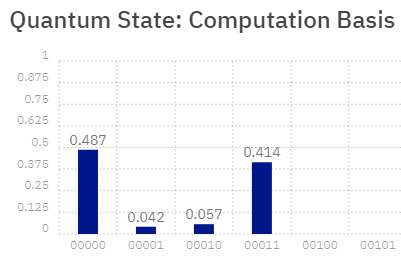
\includegraphics[scale=0.6]{ibmq1.png}
\end{figure}
\end{frame}


%%%%%%%%%%%%%%%%%%%%%%%%%%%%%%%%%%%%%%%%%%%%%%%%%%%%%%%%%%%%%%%%%%%%%%%%%

\begin{frame}
\frametitle{Tensor Product}
\pause
$\otimes$ and $\boxtimes$ are really ``the same!'' \pause $\rightarrow$ Tensor products.\\
$\,$\\
\pause
Why tensor product? \pause
\begin{block}{Postulate (QM): }
	The state space of a composite physical system is the \textit{tensor product} of the state spaces of the component physical systems.
\end{block}


\end{frame}


\begin{frame}[fragile]
\frametitle{Tensor Product}
\pause
\begin{center}
	\begin{tikzcd}[row sep=15ex, column sep=20ex]
		\V \otimes \W  \arrow[r, "linear"', "\hat{f}"]  & \X
		\\ \V \times \W \arrow[ur, "f", "bilinear"'] \arrow[u, hook, "\phi"]
	\end{tikzcd}
\end{center}

\pause 

\begin{block}{Roughly speaking...}

Giving the $\hat{f} : \V\otimes \W \lin \X$ is the same as giving $f : \V\times \W \stackrel{\text{bilinear}}{\longrightarrow} \X$. \\
$f = \hat{f}\circ \phi$
\end{block}


\end{frame}


\begin{frame}[fragile]
\frametitle{Tensor Product}
If the target space $\X$ is $\V \otimes \W$. $\lag$ is an operator on $\V$, $\M$ on $\W$,
\pause
\begin{center}
	\begin{tikzcd}[row sep=15ex, column sep=20ex]
		\V \otimes \W  \arrow[r, "linear"', "\hat{f}"]  & \V\otimes \W
		\\ \V \times \W \arrow[ur, "f", "bilinear"'] \arrow[u, hook, "\phi"]
	\end{tikzcd}
\end{center} 

 \onslide<5->{$\rightarrow$ by uniqueness}
\begin{align*}
\onslide<4->{(\lag\otimes \M)(v\otimes w)} \onslide<5->{=} \onslide<3->{\lag[v]\otimes \M[w]}
\end{align*} 

\end{frame}






\begin{frame}[fragile]
\frametitle{Tensor Product \& Kronecker Product}
\pause
$\nu$ a basis for $\V$, $\omega$ for $\W$ $\rightarrow$ can make a basis $\tau$ for $\V\otimes \W$
\pause
\begin{center}
	\begin{tikzcd}[row sep=15ex, column sep=20ex]
		\V \otimes \W  \arrow[r, "linear"', "\lag\otimes \mathcal{M}"] \arrow[d, "\{\,\}_\tau"] & \V\otimes \W
		\\ \mathbb{C}^{nm}   \arrow[r, "linear"', "{[}\lag\otimes \mathcal{M}{]}_{\tau\leftarrow\tau}"] & \mathbb{C}^{nm}  \arrow[u, "\A_\tau"]
	\end{tikzcd}
\end{center}
\pause
\begin{align*}
\boxed{[\lag\otimes \M]_{\tau\leftarrow \tau} = [\lag]_{\nu\leftarrow\nu} \otimes [\M]_{\omega\leftarrow\omega}}
\end{align*}
%\pause
%$\rightarrow$ Can calculate this via the Kronecker product
\end{frame}







\section{Recap}

\begin{frame}
\frametitle{Recap}
\begin{itemize}
\pause
\item How a 2-qubit entangling circuit works
\pause
\item Qubits, quantum gates as matrices
\pause
\item Kronecker product
\pause
\item Entanglement
\pause
\item Tensor product
\pause
\item Why quantum computer?
\end{itemize}

\end{frame}

\begin{frame}
\frametitle{References}



\bibliographystyle{amsalpha}
\bibliography{references}{}



\end{frame}









 
\end{document}
